\documentclass[12pt]{article}
%Gummi|065|=)
\title{\textbf{Arreglos y parametros de los amplificadores clase A}}
\author{Guzman Vazquez Jaime Alan\\
Sistemas electronicos de interfaz}
\date{0ctubre 1}
\usepackage{graphicx}
\begin{document}
\begin{figure}[htp]
\centering

\includegraphics[scale=1.00]{/home/emile/Escritorio/guzman.vazquez.jaime.alan.yamil/tareas/EV_2_2_explicar_los_arreglos_y_parametros_de_los_amplificadores_clase_A./imagenes/índice.png}
\caption{}
\label{}
\end{figure}
\maketitle
\section{amplificadores clase A.}
Los amplificadores de la clase A son aquellos cuyas etapas consumen corrientes altas y continuas desde su fuente de alimentacion independientemente si existe señal o no.\\
Las caracteristicas principales de estos amplificadores es que a menudo consisten en un transistor de salida conectado al positivo y un transistor de corriente constante conectado de la salida al negativo de la fuente de alimentacion.\\\\
Las ventajas de este tipo de amplificadores  es que debido a su clasificacion A estos tienen una etapa de salida con una corriente  de polarizacion mayor que la maxima corriente de salida que dan, De tal forma que los transistores de salida siempre estan consumiendo corriente. la gran ventaja de la clase A es que es casi lineal y en consecuencia la distorcion es menor.\\\\
Las desventajas de este tipo de amplificacion es que es poco eficiente, se requiere un amplificador clase A muy grande para dar 50w y este se podra a alta temperatura ademas de jalar grandes cantidades de corriente.\\  

\begin{figure}[htp]
\centering
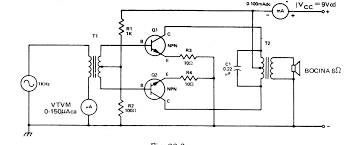
\includegraphics[scale=0.50]{imagenes/images.png}
\caption{esquematico de amplificador clase A}
\label{}
\end{figure}
\begin{figure}[htp]
\centering
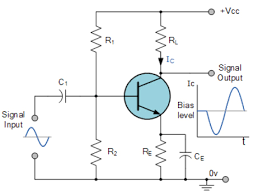
\includegraphics[scale=0.50]{imagenes/1.png}
\caption{esquematico amplificador.}
\label{}
\end{figure}
Esta es una breve descripcion de los amplificadores y algunas ventajas y desventajas de estos, a continuacion describiremos su funcion asi como los tipos de amplificadores que existen.\\\\

\maketitle
\section{Funcionamiento}
Un amplificador de clase A tiene como funcion principal el que la señal de salida sea una señal como la que entro pero amplificada y sin distorsion, en este caso la maxima señal de salida se obtendra cuando el punto estatico este coincidiendo con el centro de la recta de carga.
Esto permite el mayor rendimiento del circuito a partir de el cual puede ser amplificado, estos son amplificadores que trabajan a onda completa mas como ya se menciono estos desperdician gran parte de su capacidad debido a su desgaste en cuanto a temperatura se refiere.


\maketitle
\section{tipos de amplificadores}
AMPLIFICADOR DE UNA SOLA ETAPA\\\\\\
Este es el tipo mas simple de circuito de amplificacion de potencia de clase A utiliza un transistor de extremo unico para su etapa de salida con la carga resistiva conectadadirectamente al terminal colector.\\ cuando el transistor se enciende, se hunde la corriente de la salida a travez del colector, lo que resulta en una copia en una caida de voltaje inevitable a travez de la resistencia del emisor, limitando asi la capacidad de salida negativa.\\
la eficiencia de estos dispositivos es de menos del 30%.\\

CONFIGURACION DEL TRANSISTOR DARLINGTON\\\\\\
La ganacia de corriente total o el valor de HFE de un dispositivo Darlington es el producto  de las dos ganacias individuales  de los transistores multiplicadas juntas  y valores muy elevados junto con las altas corrientes de colector son posibles en comparacion con un solo circuito de transistor.\\


AMPLIFICADOR CONECTADO A TRANSFORMADOR.\\\\\\

Como la corriente del colector, Ic se reduce por debajo del punto Q quieto establecido por la tension de polarizacion basica, debido a las variaciones en la corriente base, el flujo magnetico magnetico en el nucleo del transformador se colapsa causando una fem inducidas en los devanados primarios del transformador. Este tiene como funcion principal el generar una tension instantanea del colector aumente a un valor doble de la tension.  


\section{Bibliografia}
electronicabasica.blogspot\\
ecured.cu\\
ft.unicamp.br.
\end{document}
